\chapter{Sample of DES SLSNe}
\label{Chapter6}
\lhead{Chapter 6. \emph{High redshift SLSN}}

\begin{figure}[H]
  \centering
  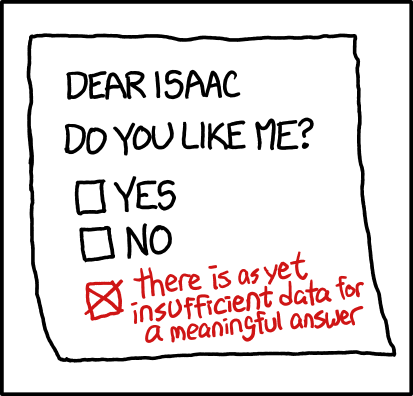
\includegraphics{Figures/xkcd/chapter6.png}
  \caption*{xkcd.com/1448}
\end{figure}

The aim of this chapter, cultumating the overall goal of this thesis, is the study of a sample of SLSNe in DES. In the previous chapters I identified SLSNe using the magnetar model approach, built an artifial sample of SLSNe, as well as numerous other classes of transients, and constructed a photometric classification of DES SN candidates. This process has identified a large sample of 500 potential SLSN candidates that, while I believe hides a large number of true SLSNe, is heavily contaminated with slowly evolving SN\,IIP.

Here, I begin by examining this dataset in order to separate the events we are interested in through a combination of visual inspection, magnetar model fitting, unsupervised ML as well as the use of the available distance measurements. Through this process I produce a `gold' sample of DES SLSN that contains XX objects with a strong degree of confidence in their classification thanks to the presence of either spectroscopic redshift. Further to this, I produce a `silver' sample containing objects with only [WRITE TYPE] classifications and `bronze' sample which is more speculative but worth exploring in the furthcoming sections.

[WRITE WHAT MORE I'VE DONE WITH THIS DATA, WHAT OBSERVATIONAL PROPERTIES HAVE I UNCOVERED]

[FINALLY MAYBE DO A QUICK RATE? I HAVE NO IDEA HOW THAT WOULD WORK BUT ITS WORTH A SHOT]

\section{Purifying the sample of SLSNe}
text

\section{Observational Properties}
text

\section{The Rate of SLSN in DES}
text

\section{Summary}
